%
%
% UCSD Doctoral Dissertation Template
% -----------------------------------
% http:\\ucsd-thesis.googlecode.com
%
%
% ----------------------------------------------------------------------
% WARNING: 
%
%  This template has not endorced by OGS or any other official entity.
%  The official formatting guide can be obtained from OGS.
%  It can be found on the web here:
%  http://grad.ucsd.edu/_files/academic-affairs/Dissertations_Theses_Formatting_Manual.pdf
%
%  No guaranty is made that this LaTeX class conforms to the official UCSD guidelines.
%  Make sure that you check the final document against the Formatting Manual.
%  
%  That being said, this class has been used successfully for publication of 
%  doctoral theses.  
%
%  The ucsd.cls class files are only valid for doctoral dissertations.
%
%
% ----------------------------------------------------------------------
% GETTING STARTED:
%
% Lots of information can be found on the project wiki:
% http://code.google.com/p/ucsd-thesis/wiki/GettingStarted
%
%
% To make a pdf from this template use the command:
%  pdflatex template
%
%
% To get started please read the comments in this template file 
% and make changes as appropriate.
%
%
% ----------------------------------------------------------------------
%
% A thesis using this template and class file was last successfully 
% submitted on 2009/03/19 (at least as far as I know).
%
% If you successfully submit a thesis with this package please let us
% know.
%
% ----------------------------------------------------------------------
% If you desire more control, please see the attached files:
%
%   * ucsd.cls    -- Class file
%   * uct10.clo   -- Configuration files for font sizes 10pt, 11pt, 12pt
%     uct11.clo                            
%     uct12.clo
%
% ----------------------------------------------------------------------



% Setup the documentclass 
% default options: 11pt, oneside, final
%
% fonts: 10pt, 11pt, 12pt -- are valid for UCSD dissertations.
% sides: oneside, twoside -- note that two-sided theses are not accepted 
%                            by OGS.
% mode: draft, final      -- draft mode switches to single spacing, 
%                            removes hyperlinks, and places a black box
%                            at every overfull hbox (check these before
%                            submission).
% chapterheads            -- Include this if you want your chapters to read:
%                              Chapter 1
%                              Title of Chapter
%
%                            instead of
%
%                              1 Title of Chapter
\documentclass[12pt,chapterheads]{ucsd}



% Include all packages you need here.  
% Some standard options are suggested below.
%
% See the project wiki for information on how to use 
% these packages. Other useful packages are also listed there.
%
%   http://code.google.com/p/ucsd-thesis/wiki/GettingStarted



%% AMS PACKAGES - Chances are you will want some or all 
%    of these if writing a dissertation that includes equations.
%  \usepackage{amsmath, amscd, amssymb, amsthm}

%% GRAPHICX - This is the standard package for 
%    including graphics for latex/pdflatex.
\usepackage{graphicx}

%% SUBFIGURE - Use this to place multiple images in a
%    single figure.  Subfigure will handle placement and
%    proper captioning (e.g. Figure 1.2(a))
% \usepackage{subfigure}

%% LATIN MODERN FONTS (replacements for Computer Modern)
% \usepackage{lmodern}
% \usepackage[T1]{fontenc}

%% INDEX
%   Uncomment the following two lines to create an index: 
\usepackage{makeidx}
\makeindex
%   You will need to uncomment the \printindex line near the
%   bibliography to display the index.  Use the command
% \index{keyword} 
%   within the text to create an entry in the index for keyword.

%% HYPERLINKS
%   To create a PDF with hyperlinks, you need to include the hyperref package.
%   THIS HAS TO BE THE LAST PACKAGE INCLUDED!
%   Note that the options plainpages=false and pdfpagelabels exist
%   to fix indexing associated with having both (ii) and (2) as pages.
%   Also, all links must be black according to OGS.
%   See: http://www.tex.ac.uk/cgi-bin/texfaq2html?label=hyperdupdest
%   Note: This may not work correctly with all DVI viewers (i.e. Yap breaks).
%   NOTE: hyperref will NOT work in draft mode, as noted above.
% \usepackage[colorlinks=true, pdfstartview=FitV, 
%             linkcolor=black, citecolor=black, 
%             urlcolor=black, plainpages=false,
%             pdfpagelabels]{hyperref}
% \hypersetup{ pdfauthor = {Your Name Here}, 
%              pdftitle = {The Title of The Dissertation}, 
%              pdfkeywords = {Keywords for Searching}, 
%              pdfcreator = {pdfLaTeX with hyperref package}, 
%              pdfproducer = {pdfLaTeX} }


\usepackage{verbatim}

\begin{document}



%% FRONT MATTER
%
%  All of the front matter.
%  This includes the title, degree, dedication, vita, abstract, etc..
%  Modify the file template_frontmatter.tex to change these pages.
%
%
% UCSD Doctoral Dissertation Template
% -----------------------------------
% http:\\ucsd-thesis.googlecode.com
%
%


%% REQUIRED FIELDS -- Replace with the values appropriate to you

% No symbols, formulas, superscripts, or Greek letters are allowed
% in your title.
\title{The Title Of The Dissertation}

\author{Your Name Here}
\degreeyear{2009}

% Master's Degree theses will NOT be formatted properly with this file.
\degreetitle{Doctor of Philosophy} 

\field{Mathematics}
\chair{Professor Chair Master}
% Uncomment the next line iff you have a Co-Chair
% \cochair{Professor Cochair Semimaster} 
%
% Or, uncomment the next line iff you have two equal Co-Chairs.
%\cochairs{Professor Chair Masterish}{Professor Chair Masterish}

%  The rest of the committee members  must be alphabetized by last name.
\othermembers{
Professor Humor Less\\ 
Professor Ironic Name\\
Professor Cirius Thinker\\
}
\numberofmembers{4} % |chair| + |cochair| + |othermembers|


%% START THE FRONTMATTER
%
\begin{frontmatter}

%% TITLE PAGES
%
%  This command generates the title, copyright, and signature pages.
%
\makefrontmatter 

%% DEDICATION
%
%  You have three choices here:
%    1. Use the ``dedication'' environment. 
%       Put in the text you want, and everything will be formated for 
%       you. You'll get a perfectly respectable dedication page.
%   
%
%    2. Use the ``mydedication'' environment.  If you don't like the
%       formatting of option 1, use this environment and format things
%       however you wish.
%
%    3. If you don't want a dedication, it's not required.
%
%
\begin{dedication} 
 To me. And you. Which equals us.
\end{dedication}

% You are responsible for formatting here.
\begin{mydedication} 
  \vspace{1in}
  \begin{flushleft}
    To me.
  \end{flushleft}
   
   \vspace{2in}
   \begin{center}
     And you.
   \end{center}

  \vspace{2in}
  \begin{flushright}
    Which equals us.
  \end{flushright}
\end{mydedication}



%% EPIGRAPH
%
%  The same choices that applied to the dedication apply here.
%

% The style file will position the text for you.
\begin{epigraph} 
  \emph{A careful quotation\\
  conveys brilliance.}\\
  ---Smarty Pants
\end{epigraph}

 % You position the text yourself.
\begin{myepigraph}
   \vfil
   \begin{center}
     \emph{A careful quotation\\
     conveys brilliance.}\\
     ---Smarty Pants
   \end{center}
 \end{myepigraph}


%% SETUP THE TABLE OF CONTENTS
%
\tableofcontents
\listoffigures  % Uncomment if you have any figures
\listoftables   % Uncomment if you have any tables



%% ACKNOWLEDGEMENTS
%
%  While technically optional, you probably have someone to thank.
%  Also, a paragraph acknowledging all coauthors and publishers (if
%  you have any) is required in the acknowledgements page and as the
%  last paragraph of text at the end of each respective chapter. See
%  the OGS Formatting Manual for more information.
%
\begin{acknowledgements} 
 Thanks to whoever deserves credit for Blacks Beach, Porters Pub, and
 every coffee shop in San Diego. 

 Thanks also to hottubs.
\end{acknowledgements}


%% VITA
%
%  A brief vita is required in a doctoral thesis. See the OGS
%  Formatting Manual for more information.
%
\begin{vitapage}
\begin{vita}
  \item[2002] B.~S. in Mathematics \emph{cum laude}, University of Southern North Dakota, Hoople
  \item[2002-2007] Graduate Teaching Assistant, University of California, San Diego
  \item[2007] Ph.~D. in Mathematics, University of California, San Diego 
\end{vita}
\begin{publications}
  \item Your Name, ``A Simple Proof Of The Riemann Hypothesis'', \emph{Annals of Math}, 314, 2007.
  \item Your Name, Euclid, ``There Are Lots Of Prime Numbers'', \emph{Journal of Primes}, 1, 300 B.C.
\end{publications}
\end{vitapage}


%% ABSTRACT
%
%  Doctoral dissertation abstracts should not exceed 350 words. 
%   The abstract may continue to a second page if necessary.
%
\begin{abstract}
  This dissertation will be abstract. 
\end{abstract}


\end{frontmatter}

%% START THE FRONTMATTER, THIS TIME WITH A Co-Chair
%
\title{The Title Of The Dissertation, But This Time A Really Really Really Long Title That Will Span More Than One Line.}

\chair{Professor Chair Master}
% Uncomment the next line iff you have a Co-Chair
\cochair{Professor Cochair Semimaster} 
%
% Or, uncomment the next line iff you have two equal Co-Chairs.
%\cochairs{Professor Chair Masterish}{Professor Chair Masterish}

%  The rest of the committee members  must be alphabetized by last name.
\othermembers{
Professor Humor Less\\ 
Professor Ironic Name\\
Professor Cirius Thinker\\
Professor Lateto Mydefense\\
}
\numberofmembers{5} % |chair| + |cochair| + |othermembers|
\begin{frontmatter}

%% TITLE PAGES
%
%  This command generates the title, copyright, and signature pages.
%
\makefrontmatter 

%% ABSTRACT
%
%  Doctoral dissertation abstracts should not exceed 350 words. 
%   The abstract may continue to a second page if necessary.
%
\begin{abstract}
  %This dissertation will be abstract. And confusing too.

 Five and Seven said nothing, but looked at Two. Two began in a low voice, `Why the fact is, you see, Miss, this here ought to have been a red rose-tree, and we put a white one in by mistake; and if the Queen was to find it out, we should all have our heads cut off, you know. So you see, Miss, we're doing our best, afore she comes, to--' At this moment Five, who had been anxiously looking across the garden, called out `The Queen! The Queen!' and the three gardeners instantly threw themselves flat upon their faces. There was a sound of many footsteps, and Alice looked round, eager to see the Queen.

First came ten soldiers carrying clubs; these were all shaped like the three gardeners, oblong and flat, with their hands and feet at the corners: next the ten courtiers; these were ornamented all over with diamonds, and walked two and two, as the soldiers did. After these came the royal children; there were ten of them, and the little dears came jumping merrily along hand in hand, in couples: they were all ornamented with hearts. Next came the guests, mostly Kings and Queens, and among them Alice recognised the White Rabbit: it was talking in a hurried nervous manner, smiling at everything that was said, and went by without noticing her. Then followed the Knave of Hearts, carrying the King's crown on a crimson velvet cushion; and, last of all this grand procession, came the King and Queen of Hearts.

\end{abstract}

\end{frontmatter}






%% DISSERTATION

% A common strategy here is to include files for each of the chapters. I.e.,
% Place the chapters is separate files: 
%   chapter1.tex, chapter2.tex
% Then use the commands:
%   \chapter{Introduction}
The loss of muscle mass with aging and disuse atrophy has been studied extensively. 
Accompanying the loss of muscle mass (\textit{sarcopenia}) is a disproportionately greater loss of muscle strength (\textit{dynapenia}) as we age~\cite{RNIGoodpaster}. 
The role of muscular and neural determinants of muscle force have been investigated in several human and animal studies~\cite{RNIBallak}.
In addition to these determinants, the role of the extracellular matrix (Figure~\ref{fig: ECM}) is also being increasingly recognized~\cite{RNIRamaswamy, RNIZhang}. 
For example, aging significantly alters proteins that transmit force both inside the muscle fibers~\cite{RNIHughes} and in the extracellular matrix~(ECM)~\cite{RNIKragstrup}, changing their content, orientation and composition. 
%*********************************************************
\begin{figure}[!ht]
\centering
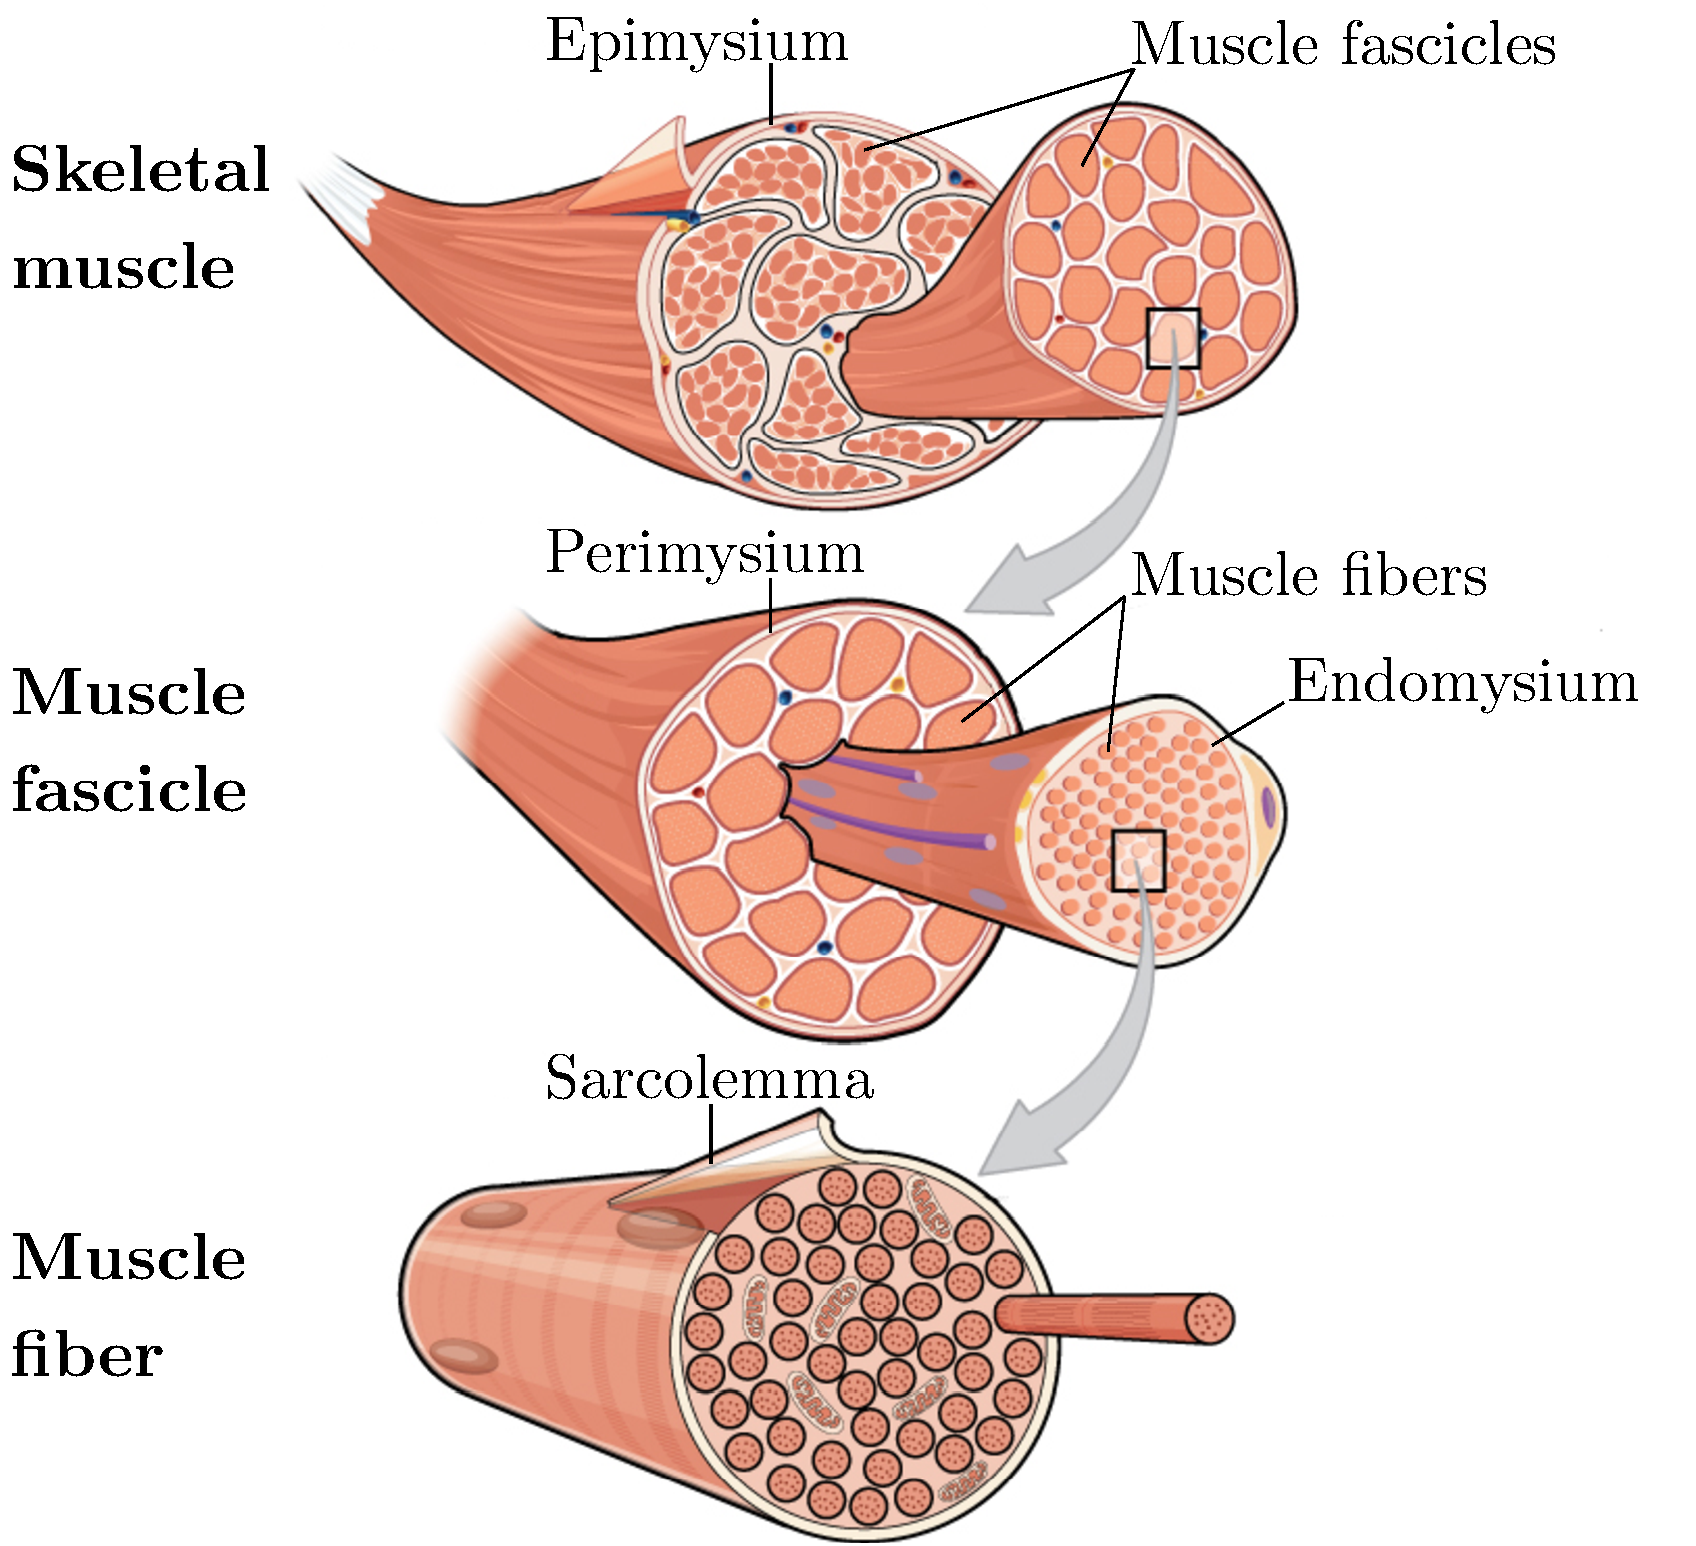
\includegraphics[scale=.4]{Figures/FIBER.pdf}
\caption[Skeletal muscle extracellular matrix]{Skeletal muscle extracellular matrix (ECM).}
\label{fig: ECM}
\end{figure}
%*********************************************************
The remodeling of the ECM may contribute to muscle weakness by impairing a muscle'��s capacity to transmit force. 
In young rodent muscles, at least 80\% of force transmission occurs laterally through the ECM~\cite{RNIHuijing}, whereas in frail old muscle, lateral transmission of force (LTF) through the ECM is reduced ~60\%~\cite{RNIRamaswamy, RNIZhang}. 
However, the contribution of the ECM to \textit{dynapenia} has never been comprehensively investigated in humans due to lack of non-invasive tools.
%-new paragraph-%

%-new paragraph-%
The non-invasive, \textit{in-vivo} nature of Magnetic Resonance Imaging (MRI) renders it particularly amenable to longitudinal studies of aging and disuse for both research and clinical purposes. 
MRI provides a unique non-invasive approach to monitor the \textit{in-vivo} changes in tissue deformation (strain or strain rate tensor) and its microarchitecture (diffusion modeleing).
%-new paragraph-%

%-new paragraph-%
My work explores age and atrophy related changes in strain rate parameters and their relationship to muscle force and to muscle structure.
Functional changes are studied by extraction of strain rate parameters from velocity encoded phase contrast images (VEPC).
Shear strain in the ECM has been postulated and validated with computational models to be the mechanism of lateral transmission of force. Thus mapping shear strain can potentially reflect changes in force transmission pathways.
It should be noted that shear strain will be influenced by the structural remodeling of the extracellular matrix.
Structural changes are studied using diffusion tensor imaging and the results are interpreted using bicompartment and random permeable barrier diffusion models.
%   %#########################################################
\chapter{Fundamentals of MRI}
%#########################################################
Among various medical imaging modalities Magnetic Resonance Imaging (MRI) is currently the most powerful technique to study structure and functions of human body \textit{in-vivo} and non-invasively at the level of the detail that is not available with any other imaging method. 
The power of MRI comes from the ability to to obtain quantitative spatial information for different types of human body tissue and fluids placed inside a strong magnetic field by manipulating Radio-frequency (RF) and gradient pulses. 
Magnetic Resonance Imaging is a fascinating combination of quantum physics, electrodynamics, advanced engineering and computation methods. 
This chapter is a short introduction to the fundamentals of MRI.
%=========================================================
\section{Larmor Precession}
%=========================================================
A charged particle placed in an external magnetic field will precess at a frequency proportional to this external field. 
In classical description magnetic dipole moment for a charged particle $\boldsymbol\mu$ is proportional to the angular momentum $\mathbf{J}$:
%.........................................................
\begin{equation}\label{eq: Classical magnetic moment}
	\boldsymbol{\mu}=\frac{q}{2m}\mathbf{J}
\end{equation}
%.........................................................
where $q$ is the charge of a particle and $m$ is its mass. 
Torque on a magnetic dipole in external magnetic filed $\mathbf{B}$ is:
%.........................................................
\begin{equation}\label{eq: Torque}
	\boldsymbol{\tau}=\frac{d\mathbf{J}}{dt}=\boldsymbol{\mu}\times\mathbf{B}=\frac{q}{2m}\mathbf{J}\times\mathbf{B}
\end{equation}
%.........................................................
Precessional frequency is then:
%.........................................................
\begin{equation}\label{eq: Classic Larmor frequency}
	\omega=\frac{d\phi}{dt}=-\frac{d\phi}{d\mathbf{J}}\cdot \frac{d\mathbf{J}}{dt}=\frac{1}{J\sin{\theta}}\cdot \frac{q}{2m}\ - J B \sin{\theta}
\end{equation}
%.........................................................
where $d\phi$ is the rotation angle and $\theta$ is the angle enclosed by angular momentum $\mathbf{J}$ and magnetic field $\mathbf{B}$:
%.........................................................
\begin{equation}\label{eq: Classic Larmor frequency 2}
	\omega=-\frac{q}{2m}\ B
\end{equation}
%.........................................................
In quantum mechanics description magnetic dipole moment is quantized:
%.........................................................
\begin{equation}\label{eq: Quantum magnetic moment}
	\boldsymbol{\mu}=\gamma\hbar \mathbf{I}
\end{equation}
%.........................................................
where  $\gamma$ is gyromagnetic ratio (for protons: $\gamma/2\pi = \SI{42.57}{\mega\hertz /\tesla}$), $\hbar = \SI{1.05e-34}{\joule \cdot \second}$ is reduced Planck constant and $\mathbf{I}$ is nuclear spin angular momentum. For each proton energy is:
%.........................................................
\begin{equation}\label{eq: Quantum energy}
	\varepsilon=-\boldsymbol{\mu}\cdot \mathbf{B}=-\gamma\hbar\mathbf{I}\cdot\mathbf{B}
\end{equation}
%.........................................................
and since there are only two possible states (magnetic moment is almost parallel or anti-parallel to the external magnetic field $\mathbf{B}$) with $ I = \pm 1/2$  the energy difference between these states is:
%.........................................................
\begin{equation}\label{eq: Quantum energy delta}
	\Delta\varepsilon=-\left(\frac{1}{2} + \frac{1}{2}\right)\gamma\hbar B
\end{equation}
%.........................................................
using Einstein-Planck relation $\Delta\varepsilon=\hbar\omega$ and Equation~\ref{eq: Quantum energy delta} the Larmor frequency:
%.........................................................
\begin{equation}\label{eq: Quantum Larmor frequency}
	\omega=-\gamma B
\end{equation} 
%.........................................................
Comparing Equations~\ref{eq: Classic Larmor frequency 2} and \ref{eq: Quantum Larmor frequency} one can see that the precessional frequency is same as the frequency of the photon that can be absorbed or emitted by proton to go from one energy state to another.
%=========================================================
\section{Population of Energy States}
%=========================================================
The signal measured in MRI is the net magnetization $\mathbf{M_{0}}$ which is a result of difference in proton energy level population density given by Boltzmann distribution:
%.........................................................
\begin{equation}\label{eq: Boltzmann distribution}
	\frac{N_{\mathrm{up}}}{N_{\mathrm{down}}}=\exp\left(\frac{-\Delta\varepsilon}{k_{B}T}\right)\approx 1 + \frac{{\gamma\hbar B}}{k_{B}T}
\end{equation}
%.........................................................
where $k_{B} = \SI{1.38e-23}{\joule \cdot {\kelvin}^{-1}}$ is Boltzmann constant the difference is then:
%.........................................................
\begin{equation} \label{eq: Population difference}
	\Delta N = \frac{N_{\mathrm{total}}}{2}\frac{\gamma\hbar B}{k_{B}T}
\end{equation}
%.........................................................
multiplying Equation~\ref{eq: Population difference} by magnetic moment $\mu = \gamma \hbar / 2$ and dividing by a total number of protons gives the equation for magnetization per unit volume:
%.........................................................
\begin{equation}\label{eq: Magnetization per volume}
	\mathbf{M_{0}}=\frac{\rho\gamma^2\hbar^2\mathbf{B}}{4k_{B}T}
\end{equation}
%.........................................................
where $\rho$ is proton density. 
From the Equation~\ref{eq: Magnetization per volume} one can see that the measured signal is directly proportional to the strength of the external magnetic field and inversely proportional to the tissue or fluid temperature. 
The direction of net magnetization is matched with the direction of the external magnetic field $\mathbf{B}$ since there are more protons in a low level energy state (aligned with external magnetic field). 
Equation~\ref{eq: Magnetization per volume} provides an estimate for the signal to be measured. 
Simple example would be magnetization for $\SI{1}{\milli\liter}$ of water at temperature $\SI{310}{\kelvin}$) placed in the $\SI{1}{\tesla}$ magnetic field. 
Calculating proton density $\rho$ of water using the Avogadro number gives:
%.........................................................
\begin{equation}\label{eq: Magnetization estimation}
	\mathbf{M_{0}}\approx \SI{3}{\milli\ampere / \meter} 
\end{equation}
%.........................................................
Compared to the strength of the external magnetic field $\mathbf{B}$ the magnetization of the tissue of interest is much smaller which makes it hard to measure when at equilibrium. 
If tipped to the transverse plane by applying RF-pulse the signal becomes distinct and easier to measure.
%=========================================================
\section{Bloch Equations}
%=========================================================
The evolution of net magnetization is described by Bloch equation~\cite{Bloch1946}:
%.........................................................
\begin{equation}\label{eq: Bloch equation}
	\frac{d\mathbf{M}}{dt}=\gamma\mathbf{M} \times \mathbf{B}
\end{equation}
%.........................................................
relaxation and diffusion terms are dropped to simplify further examination. To flip magnetization to the plane perpendicular to the direction of the applied strong magnetic field and produce transverse magnetization an RF-pulse should be applied. A common approach is to switch from laboratory reference frame defined with respect to the scanner to the frame rotating at some constant angular frequency $\Omega$. Magnetic field $\mathbf{B}$ in the laboratory reference frame can be chosen as following form:
%.........................................................
\begin{equation}\label{eq: External B field}
	\mathbf{B}=\hat{x}B_{1}(t)\cos{\omega_{\text{rf}} t}-\hat{y}B_{1}(t)\sin{\omega_{\text{rf}} t} +\hat{z}B_0
\end{equation}
%.........................................................
where $B_0$ is constant strong magnetic field aligned with the $z$-axis and $B_1$ is the time-varying component in the transverse plane. 
Rewriting Bloch equation using Equation~\ref{eq: External B field}:
%.........................................................
\begin{equation}\label{eq: Bloch equation lab frame}
\left(\frac{d\mathbf{M}}{dt}\right)_{\text{lab}}=\gamma\mathbf{M}\times\biggl[\hat{x}B_1(t)\cos{\omega_{\text{rf}}t}-\hat{y}\sin{\omega_{\text{rf}}t}+\hat{z}B_0\biggr]
\end{equation}\\
%.........................................................
In matrix form and frame of reference rotating at constant frequency $\Omega$ time-varying field $\mathbf{B_{1}}$ is the following:
%.........................................................
\begin{equation}\label{eq: External B field rotating frame}
\begin{bmatrix}
    B_{1,x}(t)\\
    B_{1,y}(t)\\
    B_{1,z}(t)\\
\end{bmatrix}_{\mathrm{rot}} = 
	\begin{bmatrix}
    \cos{\Omega t} & -\sin{\Omega t} & 0\\
    \sin{\Omega t} & \cos{\Omega t} & 0\\
    0 & 0 & 1\\
	\end{bmatrix}
	\begin{bmatrix}
    \phantom{-}B_{1}(t)\cos{\omega_{\text{rf}} t}\\
    -B_{1}(t)\sin{\omega_{\text{rf}} t}\\
    0\\
	\end{bmatrix}
\end{equation}
%.........................................................
after performing multiplication and making use of trigonometric identities the transverse component $\mathbf{B_{1}}$ in the rotating frame of reference is:
%.........................................................
\begin{equation}\label{eq: External B field rotating frame 2}
	\mathbf{B_{1}}_{\mathrm{rot}}(t)=
	\begin{bmatrix}
	B_{1}(t) \cos(\Omega -\omega_{\text{rf}})t\\
	B_{1}(t) \sin(\Omega -\omega_{\text{rf}})t\\
	0	
	\end{bmatrix}
\end{equation}
%.........................................................
Closely following~\cite{Slichter1990, RNDT24} Equation~\ref{eq: Bloch equation lab frame} the Bloch equation in the rotating frame becomes: 
%.........................................................
\begin{equation}\label{eq: Bloch equation rot}
\begin{split}
	\left(\frac{d\mathbf{M}}{dt}\right)_{\text{rot}} &=\left(\frac{d\mathbf{M}}{dt}\right)_{\text{lab}} + \Omega \hat{z} \times \mathbf{M} =\\ \\
	&= \gamma\mathbf{M}\times\biggl[B_1(t)(\hat{x}\cos{(\omega_{\text{rf}}-\Omega)}t-\hat{y}\sin{(\omega_{\text{rf}}-\Omega)t)}+
		 \hat{z}\left(B_0-\frac{\Omega}{\gamma}\right)\biggr]
\end{split}	
\end{equation}\\ \\
%.........................................................
Carrying out vector cross product the system of equation in scalar form:
%.........................................................
\begin{equation}\label{eq: scalar form of Bloch}
\begin{aligned}
	\left(\frac{M_x}{dt}\right)_\mathrm{rot} &= \gamma M_y\left(B_0-\frac{\Omega}{\gamma}\right)+\gamma M_zB_1(t)\sin(\omega_{\text{rf}}-\Omega)t\\
	\left(\frac{M_y}{dt}\right)_\mathrm{rot} &= -\gamma M_x\left(B_0-\frac{\Omega}{\gamma}\right)+\gamma M_zB_1(t)\cos(\omega_{\text{rf}}-\Omega)t\\
	\left(\frac{M_z}{dt}\right)_\mathrm{rot} &= -\gamma M_xB_1(t)\sin(\omega_{\text{rf}}-\Omega)t - \gamma M_yB_1(t)\cos(\omega_{\text{rf}}-\Omega)t
\end{aligned}
\end{equation}
%.........................................................
Three special cases are:
\begin{itemize}
	\item \textit{RF reference frame: }$\Omega=\omega_{\text{rf}}$\\
	Frequency of rotating frame $\Omega$ same as the RF-pulse frequency $\omega_{\mathrm{rf}}$
%.........................................................
\begin{equation}\label{eq: Bloch case 1}
	\left(\frac{d\mathbf{M}}{dt}\right)_{\text{rot}}=\gamma\mathbf{M}\times\left[\hat{x}B_1(t)+\hat{z}\left(B_0-\frac{\omega_{\text{rf}}}{\gamma}\right)\right]	
\end{equation}
%.........................................................
here $B_1$ field is stationary. and due to the choice for $\mathbf{B}$ in Equation~\ref{eq: External B field} the filed $B_1$ is oriented along $x$ axis. 
In general $B_1$ field can have both $x$ and $y$ component.
\item \textit{Larmor reference frame: }$\Omega=\omega$\\
Rotating frame frequency $\Omega$ equals Larmor frequency $\omega = \gamma B_{0}$
%.........................................................
\begin{equation}\label{eq: Bloch case 2}
	\left(\frac{d\mathbf{M}}{dt}\right)_{\text{rot}}=\gamma\mathbf{M}\times\left[B_1(t)(\hat{x}\cos{(\omega_{\text{rf}}-\omega)}t-\hat{y}\sin{(\omega_{\text{rf}}-\omega)t)}\right]
\end{equation}
%.........................................................
in this case the am$B_0$ filed is eliminated.
\item \textit{Resonance case:} $\omega=\omega_{\text{rf}}=\omega_{0}$
%.........................................................
\begin{equation}\label{eq: Bloch case 3}
	\left(\frac{d\mathbf{M}}{dt}\right)_{\text{rot}}=\gamma\mathbf{M}\times \hat{x}B_1(t)
\end{equation}
%.........................................................
\end{itemize}
Rotating reference frame vastly simplifies the study of the time evolution of net magnetization by transforming rapidly oscillating RF field into the time-dependent field $B_1(t)$. 
Since $x$ and $y$ components of magnetization is of the most interest a complex magnetization $\bar{M}$ is usually introduced:
%.........................................................
\begin{equation}\label{eq: Transverse magnetization}
	\bar{M}=M_x+iM_y
\end{equation}
%.........................................................
which simplifies Equation~\ref{eq: Bloch equation rot} and gives the following compact form useful in solving for transverse components of magnetization after RF excitation pulse:
%.........................................................
\begin{equation}\label{eq: Bloch transverse}
	\left(\frac{d\bar{M}}{dt}\right)_\mathrm{rot}=-i\gamma\bar{M}\left(B_0-\frac{\Omega}{\gamma}\right)+i\gamma M_z
B_1(t)e^{-i(\omega_{\mathrm{rf}}-\Omega)t}
\end{equation}
%.........................................................
%=========================================================
\section{Building Blocks of MRI Pulse Sequences}
%=========================================================
An MRI pulse sequence is a set of programmed time-varying magnetic field pulses applied to the object of study placed inside an MRI system. 
There are two categories of pulses: 
\begin{itemize}
\item \textit{RF-pulses}: used for a number of different purposes, primarily to create measurable signal (excitation), form an echo for the signal lost during free induction decay (refocusing), selectively null the signal for certain types of tissues (inversion).
\item \textit{Gradients}: the major purpose is to create linear variation in the external magnetic field that can be exploited to spatially encode Magnetic Resonance (MR) signal, which is further reconstructed into an image (imaging gradients), control signal phase due to motion (motion-sensitizing) and various correction gradients reducing imaging artifacts~\cite{RNDT24} such as crusher gradients, eddy-current compensation and spoiler gradients. 
\end{itemize}
An infinite number of shapes for RF-pulses and gradients can be used in MRI~\cite{RNDT24, Brown:2014uy} in this section my focus is on those pulses that I used in my experiments.
%~~~~~~~~~~~~~~~~~~~~~~~~~~~~~~~~~~~~~~~~~~~~~~~~~~~~~~~~~
\subsection{RF-pulses}
%~~~~~~~~~~~~~~~~~~~~~~~~~~~~~~~~~~~~~~~~~~~~~~~~~~~~~~~~~
Every MRI pulse sequence must have at least one excitation RF-pulse. 
The purpose of excitation RF-pulse is to flip the magnetization vector $\mathbf{M}$ to allow measurements of MR signal. 
Hence flip angle $\theta$ is the major characteristics of the RF excitation pulses:
%.........................................................
\begin{equation}\label{eq: Flip Angle}
\theta (t) = \gamma \int \limits_{0}^t dt' B_{1}(t')
\end{equation}
%.........................................................
For spin-echo sequence~\cite{Hahn} a flip angle of $\SI{90}{\degree}$ is used while gradient echo sequences utilize a range of values $5-\SI{70}{\degree}$~\cite{RNDT24}.
To calculate magnetization after applying RF-pulse Equation~\ref{eq: Bloch transverse} is used leading to the solution given in~\cite{Joseph:1998fo}:
%.........................................................
\begin{equation}\label{eq: Bloch RF solution}
	\bar{M}\left( t \right) = i \gamma e^{-i\Delta\omega t} \int\limits_{0}^t dt' M_z\left( t' \right) B_1 (t')e^{i\Delta\omega t'}
\end{equation}
%.........................................................
where $\Delta \omega$ is off resonance angular frequency offset. 
This equation states that transverse complex magnetization is directly proportional to inverse Fourier transform of the product of longitudinal component of the magnetization $M_z$ and strength of the magnetic field $B_1$. 
Since $M_z$ is not constant while RF-pulse is applied a small flip angle approximation is usually used ($M_z \approx M_0$)~\cite{RNDT24} resulting in:
%.........................................................
\begin{equation}\label{eq: flip angle dependency}
	\sin{\theta} (\Delta \omega) \approx \theta (\Delta \omega)  \approx \pm \gamma \left| \int\limits_{0}^t dt' B_1 (t')e^{i\Delta\omega t'} \right|
\end{equation}
%.........................................................
Which means that the slice profile can be calculated by performing inverse Fourier transformation of the RF waveform, subject to low flip angle $\theta$. 
Another important characteristics of the RF-pulse is the carrier wave frequency usually chosen at or near Larmor frequency. 
Currently full body human scanners have the $\mathbf{B_0}$ field strength up to $\SI{7}{\tesla}$~\cite{Nowogrodzki:2018eb} giving the RF-pulses frequency range within $1 - \SI{300}{\MHz}$ for $\mathrm{^1H}$ imaging.
%---------------------------------------------------------
\subsubsection{SINC pulses}
%---------------------------------------------------------
One of the most common choice for an excitation RF-pulse is SINC pulse. 
The RF envelope of SINC pulse can be written as following:
%.........................................................
\begin{equation}\label{eq: SINC}
\begin{aligned}
B_1(t) = \begin{cases} A t_0 \dfrac{\sin \left( \tfrac{\pi t}{t_0}\right)}{\pi t},& -N_L t_0 \leq t \leq N_R t_0\\
0,& \mathrm{elsewhere}
\end{cases}
\end{aligned}
\end{equation}
%.........................................................
where $A$ is the amplitude at $t = 0$, and $N_L$ and $N_R$  are the number of zero-crossings in the SINC pulse to the left and fight of the central peak, respectively. 
%~~~~~~~~~~~~~~~~~~~~~~~~~~~~~~~~~~~~~~~~~~~~~~~~~~~~~~~~~
If flip angle is small and the pulse is applied for infinitely long time it will result in a slice profile described by rect($\Delta \omega$) function. 
Infinitely-long pulses are obviously impractical thus SINC pulse is usually truncated and apodized. 
It is primarily used for selective excitation, saturation and refocusing. 
Greatest advantage of SINC pulse is its uniform slice profile.
%--------------------------------------------------------- 
\subsubsection{The Shinnar-Le Roux (SLR) pulse}
%---------------------------------------------------------
SLR pulse design algorithm~\cite{Leroux:1990tk} allows to calculate parameters of RF-pulse from a given slice profile and  the orientation of magnetization vector $\mathbf{M}$. 
The algorithm is based on two key concepts: rotations in three-dimensional space and hard pulse approximation~\cite{RNDT24}. 
In three dimensions rotations are equivalently represented by $\mathbf{SO(3)}$ or $\mathbf{SU(2)}$ groups. 
In $\mathbf{SU(2)}$ representation the rotation matrix $\mathbf{Q}$ is:
%.........................................................
\begin{equation}\label{eq: Rotation matrix Q}
\mathbf{Q} = 
	\begin{bmatrix}
    \alpha & -\beta^*\\
    \beta & \alpha^*\\
   	\end{bmatrix}
\end{equation}
%.........................................................
where $\alpha, \beta$ are Cayley-Klein parameters. 
Matrix $\mathbf{Q}$ contains total of four real numbers which together with three rotation angles needed to describe rotation in three dimensions results into a single constraint obtained from matrix $\mathbf{Q}$ being unitary:
%.........................................................
\begin{equation}\label{eq: C-K normalization}
\alpha \alpha^*+\beta\beta^* = 1
\end{equation}
%.........................................................
The total rotation as a result of multiple pulses is given:
%.........................................................
\begin{equation}\label{eq: Q rotations}
\mathbf{Q} = \mathbf{Q}_{i}\mathbf{Q}_{i-1}\cdots\mathbf{Q}_{1}
\end{equation}
%.........................................................
Hard pulse approximation allows the soft pulse to be approximated by a set of hard pulses separated by free precession time~(Figure~\ref{fig:SLR}).
%*********************************************************
\begin{figure}[!ht]
\vspace{+0.2cm}
\centering
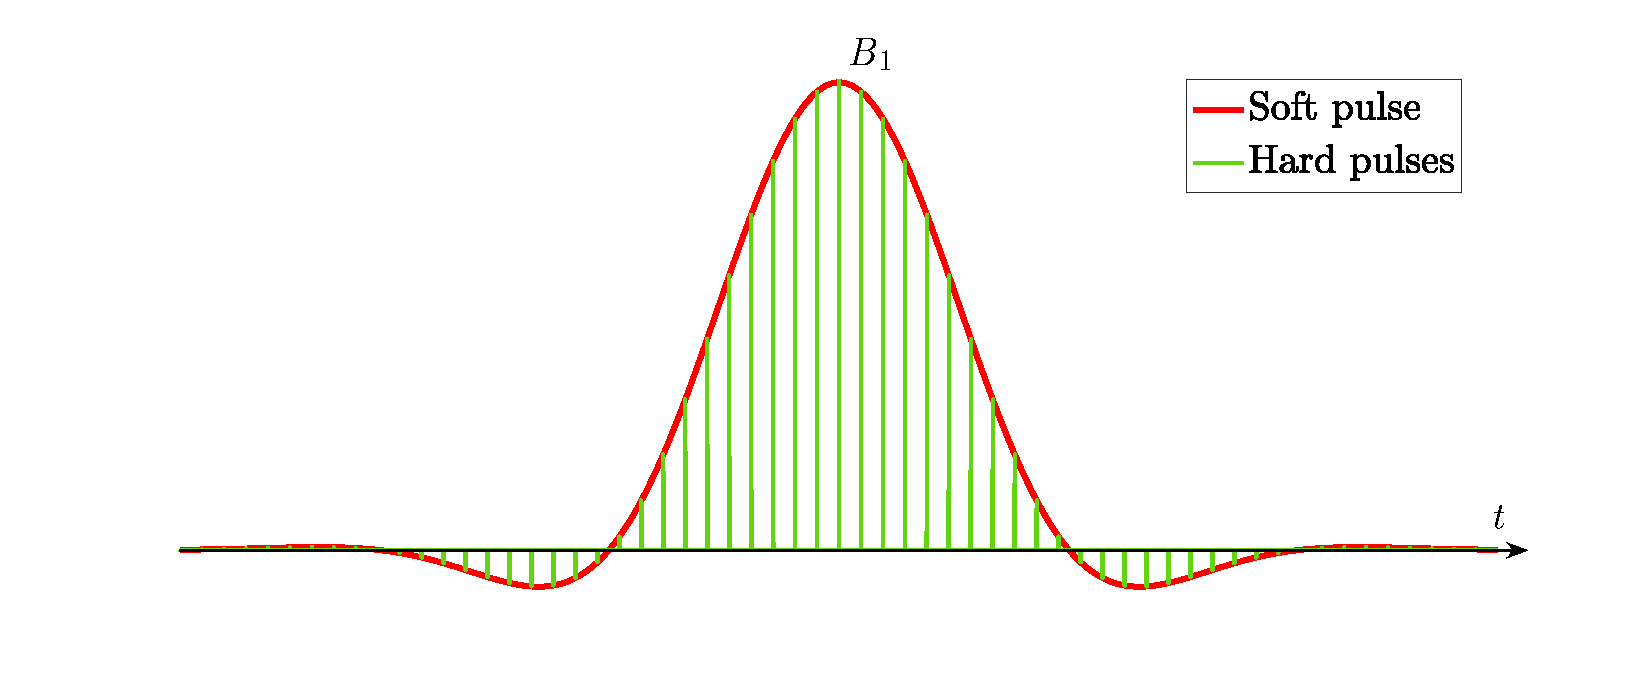
\includegraphics[scale=0.45]{Figures/SLR.pdf}
\caption[Hard pulse approximation]{Hard pulse approximation.}
\label{fig:SLR}
\end{figure}
%*********************************************************
The effect from a series of hard pulses is approximated by series of two consecutive rotations. 
The first rotation being free precession due to local gradient field by an angle $-\gamma G x \Delta t$ and the second being the rotation about applied RF vector by an angle $-\gamma B_1 \Delta t$~\cite{Pauly:1991ge}. 
Representing the $j$-th state after two consecutive rotations by spinor $s_j$ gives:
%.........................................................
\begin{equation}\label{eq: SLR j-th rotation}
s_j =
\begin{bmatrix}
    \alpha_j\\
    \beta_j\\
\end{bmatrix} = 
	\begin{bmatrix}
    C_j & -S_j^*\\
    S_j & \phantom{-}C_j\\
	\end{bmatrix}
	\begin{bmatrix}
    z^{1/2} & 0\\
    0 & z^{-1/2}\\
	\end{bmatrix}
	\begin{bmatrix}
    \alpha_{j-1}\\
    \beta_{j-1}\\
	\end{bmatrix}
\end{equation}
%.........................................................
where:
%.........................................................
\begin{equation}\label{eq: SLR two rotations}
\begin{aligned}
C_j &= \cos(\gamma \vert B_{1,j} \vert \Delta t /2) \\
S_j &= i e^{i \angle B_{1,j} }\sin(\gamma \vert B_{1,j} \vert \Delta t /2) \\
z &= e^{i \gamma G x \Delta t}
\end{aligned}
\end{equation}
%.........................................................
After N hard pulses are applied N-th state is given:
%.........................................................
\begin{equation}\label{eq: SLR rotation N}
s_N = z^{N/2}
\begin{bmatrix}
    A_N(z)\\
    B_N(z)\\
\end{bmatrix}
\end{equation}
%.........................................................
where $A_N(z)$ and $B_N(z)$ are two polynomials:
%.........................................................
\begin{equation}\label{eq: SLR rotation N}
\begin{aligned}
	A_N(z) & = \sum\limits_{n-1}^{j=0}\alpha_{j}z^{-j}\\[1mm]
	B_N(z) & = \sum\limits_{n-1}^{j=0}\beta_{j}z^{-j}
\end{aligned}
\end{equation}
%.........................................................
these polynomials must also satisfy normalization condition, which follows from Equation~\ref{eq: C-K normalization}:
%.........................................................
\begin{equation}\label{eq: C-K normalization polynom}
|A_N(z)|^2 + |B_N(z)|^2 = 1
\end{equation}
%.........................................................
Thus RF-pulse design becomes the inverse SLR transformation problem, where the profile of RF-pulse is calculated from the set of polynomials Equation~\ref{eq: SLR rotation N} that represent the initial and final state of the magnetization vector $\mathbf{M}$. 
The only missing element at this stage is interpretation of $\mathbf{SU(2)}$ results in terms of $\mathbf{SO(3)}$ since the quantity of interest is magnetization, which is a real three-dimensional vector. 
In $\mathbf{SO(3)}$ representation~\cite{1955PhRevJaynes}, components of the magnetization vector are given by the following equation:
%.........................................................
\begin{equation}\label{eq: PauliSO3_mag}
\begin{bmatrix}
    \bar{M}\phantom{^*}(+)\\
    \bar{M}^{*}(+)\\
    {M}_{z}(+)\\
\end{bmatrix} = 
	\begin{bmatrix}
    (\alpha^*)^2 & -\beta^2 & 2\alpha^*\beta\\
    -(\beta^*)^2 & \alpha^2 & 2\alpha\beta^*\\
    -(\alpha\beta)^* & -\alpha\beta & \alpha\alpha^*-\beta\beta^*\\
	\end{bmatrix}
	\begin{bmatrix}
    \bar{M}\phantom{^*}(-)\\
    \bar{M}^{*}(-)\\
    {M}_{z}(-)\\
    \end{bmatrix}
\end{equation}
%.........................................................
Using Equation~\ref{eq: PauliSO3_mag} the components of magnetization vector for three most interesting special cases of given initial conditions can be summarized in a Table~\ref{tab: SLR-Table}.
%=========================================================
\begin{table}[!htb]
\vspace{+0.2cm}
\caption[Magnetization vector response to Shinnar-Le Roux RF-pulses]{Magnetization vector response to Shinnar-Le Roux RF-pulses.}
\label{tab: SLR-Table}
\begin{center}
\begin{tabular}{@{}lcc@{}}
\toprule[1pt]\midrule[0.3pt]
Pulse Type               & \multicolumn{1}{c}{\begin{tabular}[c]{@{}c@{}}Initial Condition\\ $(M_x, M_y, M_z)$\end{tabular}} & Final State \\ \midrule
Excitation or saturation &     (0, 0, $M_0$)              &    \begin{tabular}[c]{@{}l@{}}$M_x=2M_0\text{Re}(\alpha^*\beta)$\\[1mm] $M_y=2M_0\text{Im}(\alpha^*\beta)$\\[1mm] $M_z=2M_0\alpha^*\beta$\end{tabular}         \\[9mm]
Inversion                &      (0, 0, $M_0$)             &     $M_z=M_0(\alpha\alpha^*-\beta\beta^*)$   \\[3mm]
Refocus &       ($\bar{M}$, $\bar{M^*}$, 0)            &        $\bar{M}=\bar{M}(\alpha^*)^2-\bar{M^*}\beta^2$     \\[1mm] \midrule[0.3pt]\toprule[1pt]
\end{tabular}
\end{center}
\vspace{-0.2cm}
\end{table}
%=========================================================

Although SLR design algorithm accounts for nonlinearity of Bloch equations the procedure should be repeated every time that the flip angle is changed. 
Among the advantages is the ability to make trade-offs between the parameters of RF-pulse, such as pulse duration, bandwidth, passband and stopband ripple, flip angle.
%---------------------------------------------------------
\subsubsection{Spectral Spatial Excitation Pulses (SPSP)}
%---------------------------------------------------------
This type of RF-pulse excites magnetization at specified location and with the specified spectral content~\cite{Schick:1998hu, Block:1997cv}. 
Among the advantages of SPSP pulses is the ability to replace two different conventional pulses as well as high tolerance to the $B_1$ field inhomogeneities. 
Signal from the SPSP pulses consist of a multiple short RF sub-pulses modulated by broad RF envelope combined with the bipolar slice-selective gradients~Figure~\ref{fig:SPSP}. 
The broad RF envelope performs spectral selection while sub-pulses and slice selective gradients are responsible for spatial selection.
%*********************************************************
\begin{figure}[!ht]
\vspace{+0.2cm}
\centering
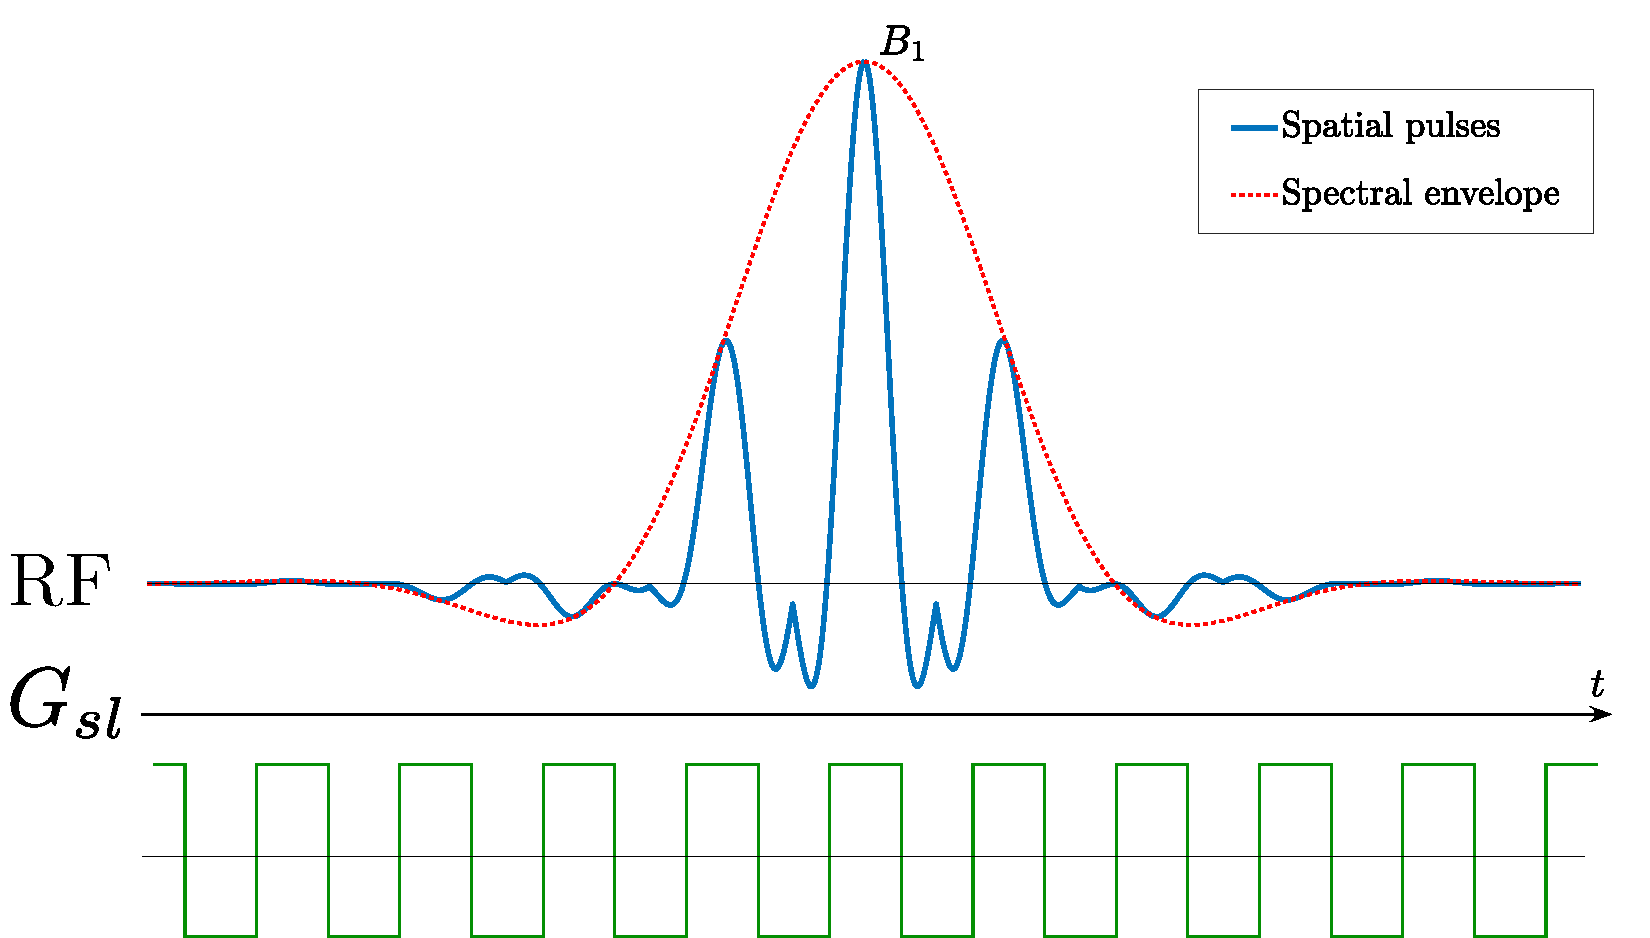
\includegraphics[scale=.35]{Figures/SPSP.pdf}
\caption[Spectral Spatial RF-pulse]{Spectral Spatial RF-pulse (SPSP).}
\label{fig:SPSP}
\end{figure}
%*********************************************************
When designing RF-pulse it is convenient to use the concept of RF \mbox{\textit{k-}space}. 
Defining $k_{\omega}$ and $k_{z}$ to be the spectral and spatial axis respectively, then:
%.........................................................
\begin{equation}\label{eq: SPSP_kspace}
\begin{aligned}
	k_z &= \frac{\gamma}{2 \pi}\int\limits_{T_{\mathrm{end}}}^t dt' \, G_{sl}(t')\\
	k_{\omega} &= T_{\mathrm{end}}-t
\end{aligned}
\end{equation}
%.........................................................	
where $G_{sl}$ is a slice selective gradient, and $T_{\mathrm{end}}$ is the end of slice rephasing gradient. 
The design of SPSP pulses includes several important stages: choice of of the slice-selection gradient form as well as it's amplitude and frequency, the placement of the desired and undesired components relative to the frequency side-lobes, the form of the RF envelope, which determines the \mbox{\textit{k-}space} weighting and thus the spatial and spectral slice profiles, the length of the pulse and the modulation of these pulses to shift them in space and frequency~\cite{RNDT24}. 
	\begin{itemize}
	\item For the slice-selection gradient oscillating trapezoidal lobes with minimal rise time and maximum amplitude are the possible choice. The oscillations are needed to sample $k_{\omega}$ axis. Such selection minimizes slice thickness since $\Delta z \propto 1/k_{z}$. 
	\item The desired and undesired components in human MRI are usually water and fat signals respectively. Simplest option is to place water at the central lobe and fat at the null between the main lobe and the first side-lobe, so called $\mathit{true-null}$ design~\cite{Meyer:1990cv}. For example a system with $B_0 = \SI{1.5}{\tesla}$ has $f = \SI{220}{\hertz}$. The required gradient modulation frequency for this method is twice the water/fat frequency difference. The period for the slice-selective gradient is then:
%.........................................................
\begin{equation}\label{eq: SPSP_period}
	T=\frac{1}{2f}=\SI{2.27}{\milli\second}
\end{equation}
%.........................................................	
The width for each trapezoidal lobe is then $T/2 = \SI{1.14}{\milli\second}$. 
Alternatively for the systems with low performance gradients hardware $\mathit{opposed-null}$ method could be used~\cite{RNDT24}. 
The period of the oscillating gradients is chosen to correspond to the closest secondary peak, increasing the width for each trapezoidal lobe by the factor of two. 
This method is however prone to partial volume artifacts, thus is less desirable to use.
\item Lastly for the choice of the RF envelope three factors are taken into account~\cite{RNDT24}.
%.........................................................
\begin{equation}\label{eq: SPSP_RF}
B_1(t)=C(\theta)|G_z(t)|A_{spec}(t)A_{spat}(k_z)
\end{equation}
where $C(\theta)$ is a normalization factor:
%.........................................................
\begin{equation}\label{eq: SPSP_C}
	C(\theta)=\frac{1}{\gamma\displaystyle\int dt A_{spec}(t)A_{spat}(k_z)}
\end{equation}
%.........................................................	
and $A_{spec}$, $A_{spat}$ is a spectral modulation envelope and spatial kernel. 
Possible choices for both $A_{spec}$ and $A_{spat}$ are SINC and SLR pulses.
\end{itemize}
A well known disadvantage of SPSP pulses is that due to the short duration of the individual sub-pulse RF they are not very spatially selective and as a result have small time-bandwidth products. 
That leads to either  broad spatial profiles transition regions or large minimum-slice thickness. 
To address these deficiencies, SPSP pulses are typically played with a high RF duty cycle~\cite{RNDT24}. 
Another issue with SPSP pulses is related to the fact that RF sub-pulses are played simultaneously with rapidly oscillating slice-selective gradients. 
If eddy currents of slice-selective gradients are not accurately compensated, the actual \mbox{\textit{k-}space} trajectory will deviate from expected and the performance of the SPSP pulse will degrade.
%~~~~~~~~~~~~~~~~~~~~~~~~~~~~~~~~~~~~~~~~~~~~~~~~~~~~~~~~~
\subsection{Gradients}
%~~~~~~~~~~~~~~~~~~~~~~~~~~~~~~~~~~~~~~~~~~~~~~~~~~~~~~~~~
While excitation RF-pulses create measurable MR signal, gradients perform its spatial and motion encoding. 
Gradients are created by pairs of coils capable of producing additional spatial linear variation to the external field $\mathbf{B}$ in each of the three orthogonal directions. 
Considering a simple case where gradient along the $x$ axis is introduced, the  magnetic field is then expressed as:
%.........................................................
\begin{equation}\label{eq: Field with gradient}
	\mathbf{B} = \mathbf{B_0} + G_x(t) \mathbf{x}
\end{equation}
%.........................................................	
As a result of the spatial linear variation of the magnetic field the precession frequency for the protons will also vary linearly according to Equations~\ref{eq: Quantum Larmor frequency}~and~\ref{eq: Field with gradient}.
 Protons subject to stronger magnetic field $\mathbf{B}$ precess faster, while those subject to weaker field precess slower~(Figure~\ref{fig: ProtonGradient}). 
%*********************************************************
\begin{figure}[!h]
\vspace{+0.2cm}
\centering
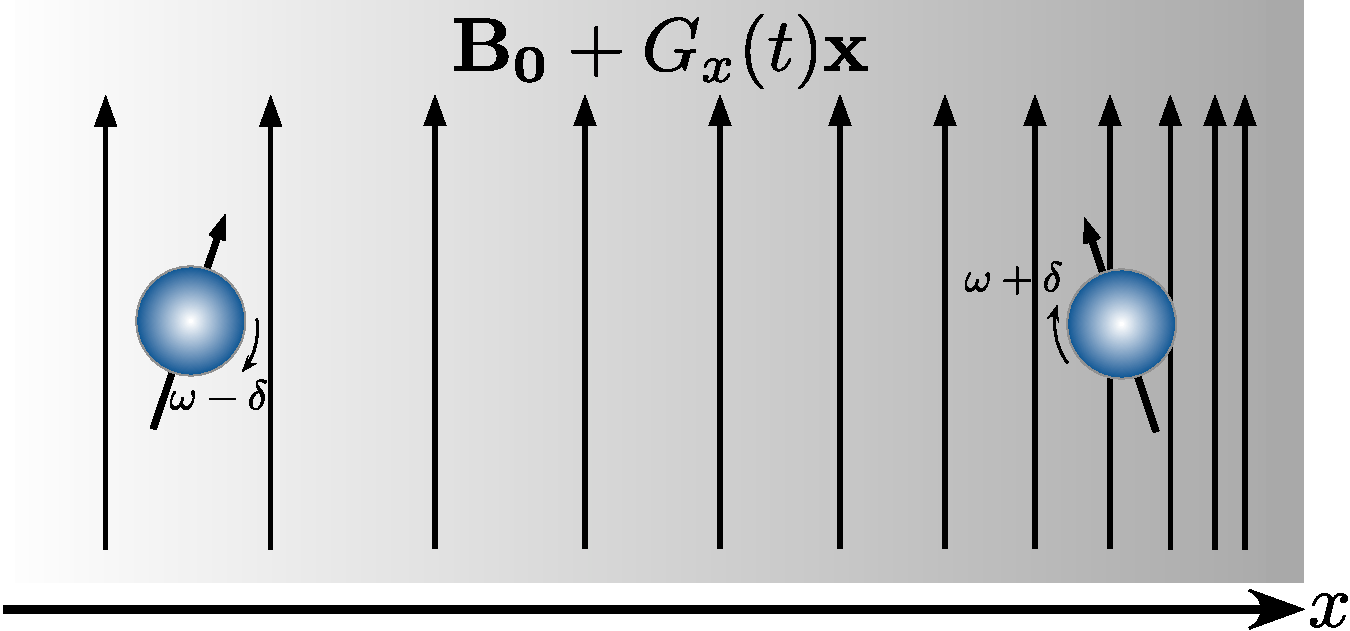
\includegraphics[scale=.4]{Figures/ProtonGradient.pdf}
\caption[Precession of protons in the magnetic field with the spatial linear gradient]{Precession of protons in the magnetic field with the spatial linear gradient applied.}
\label{fig: ProtonGradient}
\end{figure}
%*********************************************************
More general definition of gradients can be given in form of Jacobian:
%.........................................................
\begin{equation}\label{eq: Gradients}
	\mathbf{G}(t) = 
	\begin{bmatrix}
    \dfrac{\partial B_x(t)}{\partial x} & \dfrac{\partial B_x(t)}{\partial y} & \dfrac{\partial B_x(t)}{\partial z}\\[8pt]
    \dfrac{\partial B_y(t)}{\partial x} & \dfrac{\partial B_y(t)}{\partial y} & \dfrac{\partial B_y(t)}{\partial z}\\[8pt]
    \dfrac{\partial B_z(t)}{\partial x} & \dfrac{\partial B_z(t)}{\partial y} & \dfrac{\partial B_z(t)}{\partial z}\\
	\end{bmatrix}
\end{equation}
%.........................................................
For most applications the desired shape of the gradient pulse is $\mathrm{rect}(t)$ function, which would allow instantaneous change in the magnetic field. 
Yet in practice rectangular gradient pulses are impossible and are commonly approximated by trapezoid. 
Two important characteristics of the gradient pulses limited by hardware capabilities are amplitude $G_{\mathrm{max}}$ and slew rate $\sigma = G_{\mathrm{max}} / \epsilon_{\mathrm{rise}}$ ~(Figure~\ref{fig: TrapGrad}).
%*********************************************************
\begin{figure}[!htb]
\vspace{+0.2cm}
\centering
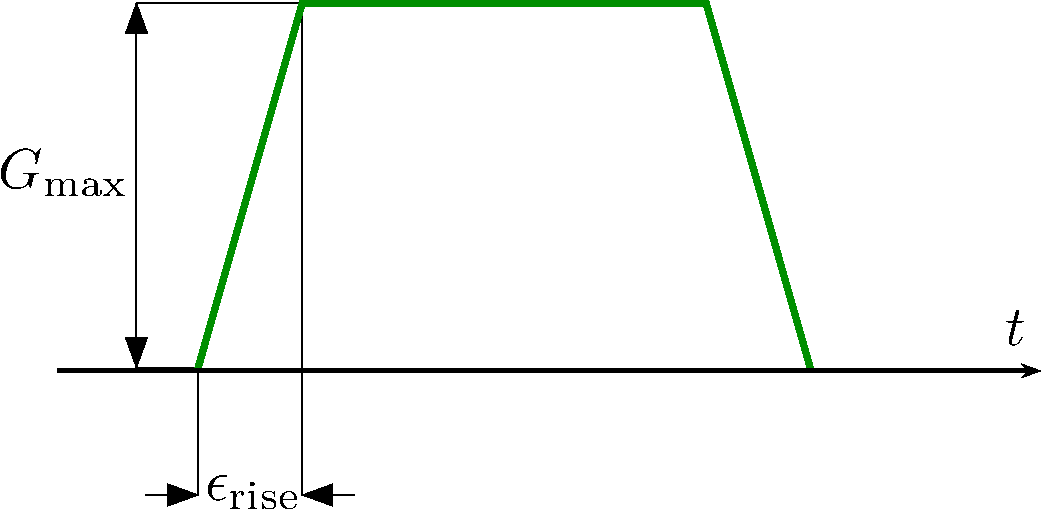
\includegraphics[scale=.48]{Figures/Trapezoid.pdf}
\caption[Trapezoid gradient shape]{Trapezoid gradient shape.}
\label{fig: TrapGrad}
\end{figure}
%*********************************************************
For modern MRI systems gradients can be applied with slew rate up to $\SI{500}{\tesla / \meter / \second}$ and amplitude up to $\SI{70}{\milli\tesla / \meter}$~\cite{Tan:2020ht}, still the full performance sometimes may not be used to avoid peripheral nerve simulation~\cite{Ham:1997is}. 
%---------------------------------------------------------
\subsubsection{Imaging gradients}
%---------------------------------------------------------
Every MRI pulse sequence incorporates imaging gradients. 
Signal is encoded spatially in 3D using three types of gradients:
\begin{itemize}
	\item \textit{Slice selection}: First imaging gradient in the pulse sequence which accompanies the initial RF excitation pulse. Slice selection gradient is applied perpendicularly to the desired slice plane and translates the band of frequencies into the desired band of locations. For the same RF-pulse band stronger slice selection gradient results in thiner slice.
	\item \textit{Phase-encoding}: Once magnetization in the selected slice is tipped to the transverse plane phase-encoding gradient is applied. Same as shown in Figure~\ref{fig: ProtonGradient} protons will experience change in angular frequency. 
%*********************************************************
\begin{figure}[!htb]
\vspace{+0.2cm}
\centering
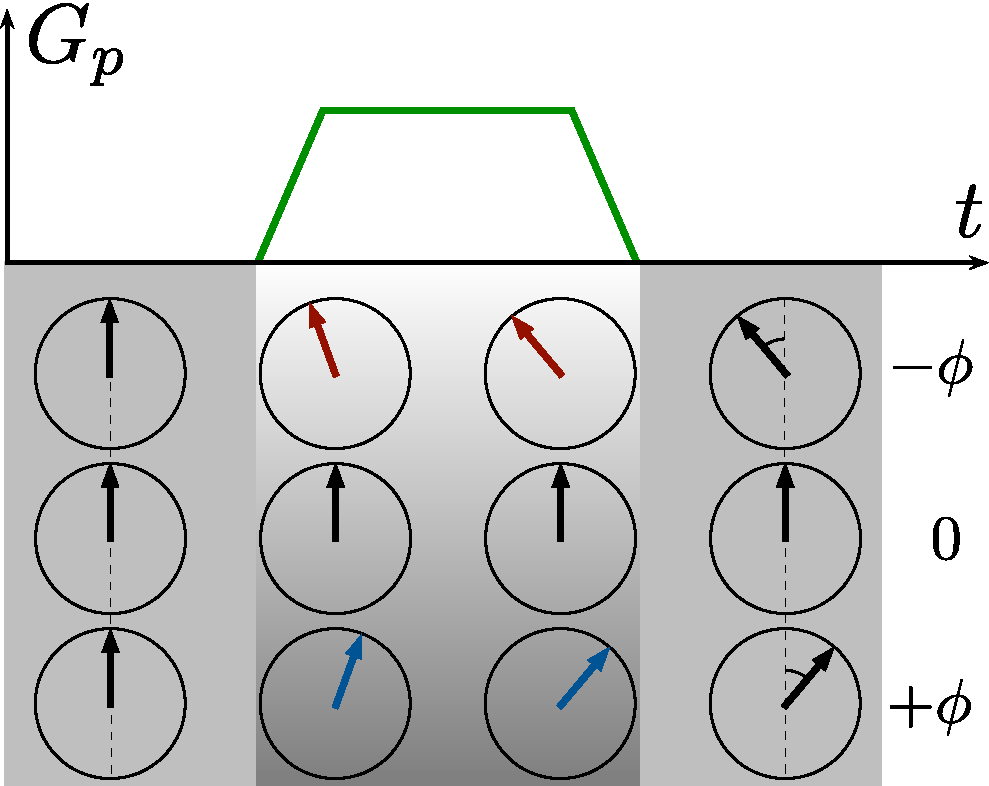
\includegraphics[scale=.45]{Figures/PhaseEncode.pdf}
\caption[Accumulated phase due to applied gradient]{Accumulated phase due to applied gradient.}
\label{fig: PhaseEncode}
\end{figure}
%********************************************************* 
	The phase-encoding gradient is then switched~off eliminating frequency variation but keeping the variation in accumulated phase intact~ Figure~\ref{fig: PhaseEncode}. Procedure should be repeated to collect data at multiple phase-encoded levels. This is achieved by varying the area under phase-encoding gradient.
	\item \textit{Frequency-encoding}: Applied continuously while the MR signal is measured it introduces spatial variation in angular frequency.\end{itemize}
Together phase- and frequency-encoding introduce an import MRI concept -- \textbf{\mbox{\textit{k-}space}}, which can be defined as a data matrix that holds phase- and frequency-encoded MR signal related to image matrix by Fourier transform.
%---------------------------------------------------------
\subsubsection{Motion-Sensitizing}
%---------------------------------------------------------
First described by Stejskal and Tanner~\cite{Stejskal} and commonly placed in the MRI sequence as a set of balanced bipolar gradients. 
These gradients are utilized to quantify the dynamics of  tissue or fluid such as diffusion and flow. 
Application of motion-sensitizing gradients for Velocity Encoded Phase-Contrast (VEPC) imaging and Diffusion Weighted Imaging (DWI) is discussed in more details in Chapters~\ref{ch: VEPC}~and~\ref{ch: Diffusion} respectively.
%---------------------------------------------------------
\subsubsection{Spoiler and Crusher}
%---------------------------------------------------------
Auxiliary gradients used to manipulate phase coherence of the magnetization vector. 
Spoiler gradients eliminate transverse magnetization by dephasing, while crushers are used to retain desired signal pathway by either dephasing or rephasing~\cite{RNDT24}. 
Crushers gradients must be used for Stimulated Echo Acquisition Mode (STEAM) which is discussed in more details in~Chapter~\ref{ch: Diffusion}.
%
% Of course, if you prefer, you can just start with
%   \chapter{My First Chapter Name}
% and start typing away.  
\chapter{Just a Test}
This is only a test.
\section{A section}
\index{latin}Lorem ipsum dolor sit amet, consectetuer adipiscing elit. Nulla odio
sem, bibendum ut, aliquam ac, facilisis id, tellus. Nam posuere pede
sit amet ipsum. Etiam dolor. In sodales eros quis pede.  Quisque sed
nulla et ligula vulputate lacinia. In venenatis, ligula id semper
feugiat, ligula odio adipiscing libero, eget mollis nunc erat id orci.
Nullam ante dolor, rutrum eget, vestibulum euismod, pulvinar at, nibh.
In sapien. Quisque ut arcu. Suspendisse potenti. Cras consequat cursus
nulla.
\subsection{More Stuff}
Blah

\chapter{How to Recognise Different Types of Trees From Quite a Long Way Away}

\section{No. 1, the Larch}
\begin{figure}[ht] 
  \centering
  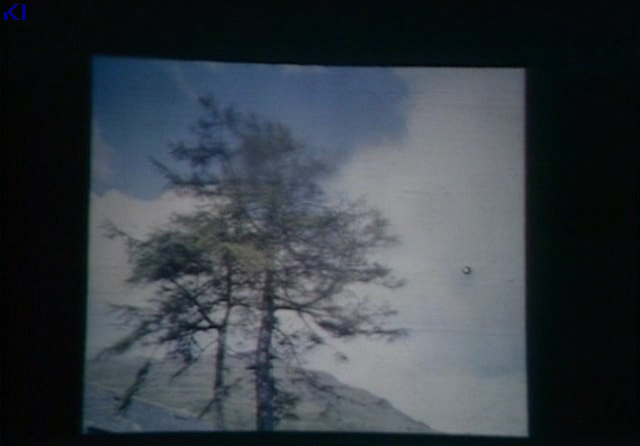
\includegraphics[width=0.8\textwidth]{larch}
  \caption{Shown is a picture of the larch as might be seen from quite a long way away.\index{Larch}}
\end{figure}

\section{And Now . . . No. 1, the Larch}
\newpage
\thispagestyle{facingcaption}
\begin{center}
\vspace*{3in}
\textbf{Figure \ref{Sideways Larch}:} Here is a caption for the Larch after you have had a wee too much to drink.

\end{center}
\newpage

\begin{figure}[hb] 
  \centering
  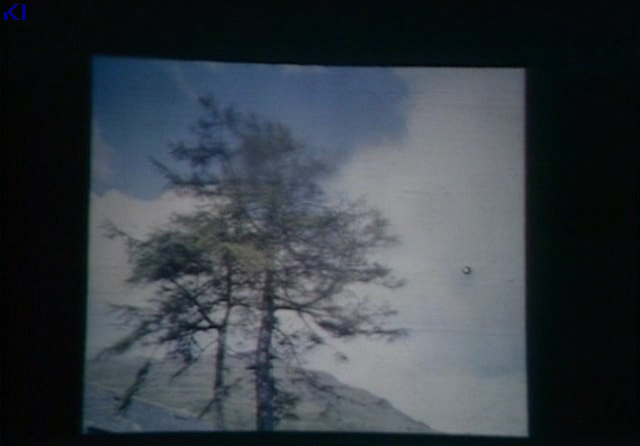
\includegraphics[width=0.8\textwidth]{larch}
  \caption[No. 1 The Larch]{Shown is a picture of the larch as might be seen from quite a long way away.\index{Larch}}\label{Sideways Larch}
\end{figure}

% Here I am testing that page breaking on the TOC works correctly.
% We never want the page break directly after a chapter entry.
\chapter{Another chapter}
\section{Some Stuff You Probably Don't Want to Read}
\section{Some Stuff You Really Don't Want to Read, it is Utterly and Completely Dull}
%\section{Now I am Just Writing Filler}
%\section{More Filler}
%\subsection{How Many Lines Am I at?}
%\subsection{Stuff}
%\section{Stuff}
%\section{Ooo-De-Laly}
%\subsection{Ooo-De-Laly, Ooo-De-Laly}
%\section{Slithy Toves}


\chapter{On the Inner Workings of a Grad Student Mind}
\section{Before Thesis Writing Has Begun}
\section{During Thesis Writing}
\section{During Thesis Formatting}
\section{After Thesis Writing}
\section{Before Defense}
\section{After Defense}

The Mock Turtle sighed deeply, and drew the back of one flapper across his eyes. He looked at Alice, and tried to speak, but for a minute or two sobs choked his voice. `Same as if he had a bone in his throat,' said the Gryphon: and it set to work shaking him and punching him in the back. At last the Mock Turtle recovered his voice, and, with tears running down his cheeks, he went on again:


\begin{verbatim}
``There's a porpoise close behind us, and he's treading on my tail.
See how eagerly the lobsters and the turtles all advance!
They are waiting on the shingle--will you come and join the dance?

Will you, won't you, 
                will you, won't you, 
                                will you join the dance?
Will you, won't you, 
                will you, won't you, 
                                won't you join the dance?''
\end{verbatim}



So Alice began telling them her adventures from the time when she first saw the White Rabbit. She was a little nervous about it just at first, the two creatures got so close to her, one on each side, and opened their eyes and mouths so very wide, but she gained courage as she went on. Her listeners were perfectly quiet till she got to the part about her repeating `You are Old, Father William,' to the Caterpillar\footnote{Which we introduced in a different thesis}, and the words all coming different, and then the Mock Turtle drew a long breath, and said `That's very curious'.

\appendix
\chapter{Final notes}
  Remove me in case of abdominal pain.





%% END MATTER
\printindex %% Uncomment to display the index
% \nocite{}  %% Put any references that you want to include in the bib 
%               but haven't cited in the braces.
% \bibliographystyle{alpha}  %% This is just my personal favorite style. 
%                              There are many others.
% \bibliography{myrefs}  %% This looks for the bibliography in myrefs.bib 
%                          which should be formatted as a bibtex file.
\end{document}

